\documentclass[12pt]{article}
\usepackage{cite}
\usepackage{graphicx}
\usepackage{subcaption}
\usepackage{caption}
\usepackage{url}

\linespread{1.25} % the equivalent of 1.5 line spacing from msword
\usepackage[a4paper, left=2.5cm,right=2.5cm,top=2.5cm,bottom=2.5cm]{geometry} % margins


\title{Web service workload prediction using deep learning - Report 3}
\date{\today}
\author{Stefan Sebastian}

\begin{document}
  \pagenumbering{gobble}
  \maketitle
  
  \newpage
  \tableofcontents
  \newpage 
  \pagenumbering{arabic}

  \section{State of the art}

  Calheiros et al.\cite{arima_prediction} apply the ARIMA model
  to cloud workload prediction. The model was evaluated using a trace of English Wikipedia resource requests
  spanning a duration of four weeks. The first three are used for training and the fourth for prediction 
  using a time window of 1 hour. The MAPE varies from 9\% to 22\% depending on the confidence interval chosen, 
  from 80 to 95 which is meant to limit the occurences of underestimations.

  Other classic timeseries models have also been applied for this task, like Brown Exponential 
  Smoothing by Mi et al.\cite{brown_prediction} obtaining a Mean Relative Error of 0.064 on 
  the France World Cup 1998 web server trace. Another classic model is Weighted Moving Average,
  applied by Aslanpour et al.\cite{wma_prediction} 
  in which recent observations are given more weight based on the Fibonacci rule, and was tested 
  on a NASA server 24h trace achieving a 5\% improvement in response time on a cloud scaling 
  simulator.

  Kumar and Singh\cite{ann_prediction} applied artificial neural networks 
  for workload prediction on a seven month log of traffic from a Saskatchewan University 
  web server and a two month one from the NASA Kennedy Space Center web server. They use 
  a classic ANN architecture : one input layer(size 10), one hidden and one output, and the model 
  is trained through the SaDE technique, which means learning its weight through evolutionary algorithms.
  The results of this model were compared to an ANN trained through backpropagation: 0.013 and 0.001 for D1 and
  D2 vs 0.265 and 0.119, using the RMSE metric over normalized data.

  CloudInsight\cite{CloudInsight} is one of the most complex models for workload prediction. It uses a technique called "council 
  of experts", meaning an ensemble of different models, in this case: classic timeseries (autoregressive, moving average, exponential smoothing),
  linear regression, and machine learning (SVM). Each model has a different prediction weight which is also learned real-time through 
  a SVM based on their accuracy on the dataset. The evaluation was done on a subset of the wikipedia trace\cite{wikidata}, on google 
  cloud data and on some generated workloads. An indicator of performance is normalized RMSE, meaning how much better it performs than 
  other models. On average it was 13\% to 27\% better than baselines (ARIMA, FFT, SVM, RSLR).
  
  A review of how deep learning methods can be applied to time series problems was created by Gamboa\cite{dl_ts}.
  The paper distinguishes between three types of problems: classification, forecasting and anomaly detection, presents
  methods for modelling them and guidance for selecting appropiate models. It also shows an improvement
  in performance over the previously existing techniques. Brownlee\cite{dlts_book} published a 
  comprehensive guide on applying MLPs, CNNs and LSTMs on various real datasets and discussed their 
  advantages over classic methods, which were used as baselines for the experiments. 

  Lin et al\cite{cnn_lstm} proposed a hybrid CNN LSTM architecture for learning trend in time series.
  It relies on on CNN to extract important features from raw timeseries data and LSTM to 
  find long range dependencies in historical data. The model was shown to outperform both CNN and LSTM 
  with around 30\% lower RMSE on 3 real world datasets.
  
  \section{Approach}
  The main goal is to find a performant model for web application 
  workload prediction, which can be later used by a proactive 
  microservice scaler. The methods used are different architectures
  of deep learning models: MLP, CNN, CNN-LSTM hybrid. The main 
  contribution of this research is the application of deep learning 
  to this specific problem and the comparison with a classic timeseries
  approach (ARIMA).

  The problem design has been influenced by the goal of integrating
  this model into a proactive microservice scaler. First of all,
  the choice of the workload measure is number of requests. The idea
  is that the scaling prediction should not influence the predicted 
  value, as would be the case with CPU or memory usage. Also this is 
  in line with research done by Jindal et al\cite{msc} who propose 
  a metric for measuring microservice performance based on number of 
  satisfied requests. Another consideration is the prediction interval.
  Taking into account the experience of Netflix\cite{scryer}, who run 
  a microservice architecture in production, the time window should be in 
  the order of minutes, so you can predict spikes and have time to deploy
  new service instances.

  A realistic workload has been used for this experiment, a wikipedia 
  trace for 12 days in september 2007. From this a subset of requests was 
  extracted (all requests for Japanese wikipedia). The subset was selected 
  in order to compare results with Kim et al.\cite{CloudInsight} which used 
  the same dataset. In order to turn a web request log file into a supervised 
  dataset the following steps were taken: create buckets which contain the 
  number of requests in a time interval, iterate over the buckets using 
  the sliding window technique\cite{sliding_window}. Basically we generate 
  training instances with input (t, t-1, ... t-n) and output (t+2). The 
  predicted value is t+2 instead of t+1 because a scaler using this model 
  would need to have a buffer window during which to deploy the services.

  After preparing the dataset two baseline models were prepared: the naive 
  approach (predict traffic in window t+2 to be traffic in t) and a classic 
  timeseries model (ARIMA). The next step was to experiment with different 
  deep learning architectures and measure the results.


  \section{Evaluation of the approach}
  \subsection{Validation and tuning}
  Model tuning and validation was done on the Japanese wikipedia trace because 
  although presenting some patterns it also has some interesting irregularities, 
  like a huge spike which is not repeated. The selected time window for tuning 
  is 10 min. todo plot of dataset

  The dataset is split into a training and testing with a ratio of 0.9.
  The validation method is k-fold Cross-Validation\cite{kfold} with k = 3, 
  which means splitting the training dataset into k equal parts, perform training
  on k - 1 and evaluation on the part left out. This process is repeated k times.
  The main idea is to not touch the testing data while tuning the model, so the 
  model will not be influenced by it.

  \subsection{Performance metrics}
  The error metrics selected for this experiment are: 
  Mean squared error(MSE), Mean absolute error(MAE)
  and Mean absolute percentage error(MAPE) as described in \cite{error_metrics} and defined in equation \ref{eq:metrics}. MSE was used as the 
  loss function for training because it tends to penalize big deviations in prediction, which is desirable for 
  our problem as we want to accurately predict traffic spikes. MAE is similar, but conceptually simpler, 
  given that each prediction error contributes in proportion to its absolute value. 
  
  MAPE is independent of the problem scale and 
  can be interpreted intuitively,  herefore can be used to give a general impression of how well a model
  performs across diferrent datasets. According to \cite{mape_values} a highly accurate forecast would 
  have MAPE lower 10\%, and a good forecast between 10 and 20\%.

  \begin{equation}
    \label{eq:metrics}
    MSE=\frac{1}{n} \sum_{i=1}^{n}(Y_i - \hat{Y_i})^2 \quad
    MAE=\frac{1}{n} \sum_{i=1}^{n}|Y_i - \hat{Y_i}| \quad
    MAPE=\frac{1}{n} \sum_{i=1}^{n}\frac{Y_i - \hat{Y_i}}{Y_i}
  \end{equation}
  


  \subsection{Baseline}
  \subsubsection{Naive baseline}
  A naive baseline is set, to get an idea if the models are useful at all. The 
  naive predictor simply states that traffic in window t+2 will be the same as 
  in the last measured window. The prediction is ploted in figure \ref{fig:baseline_pred}
  and achieves MSE: 20233320.341, MAE: 3577.844, MAPE: 7.106.

  \begin{figure}
    \centering
    \begin{subfigure}[b]{0.48\linewidth}
      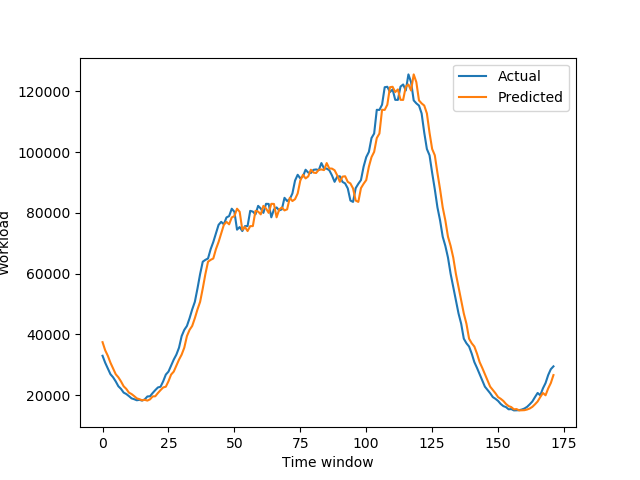
\includegraphics[width=\linewidth]{resources/baseline/naive_predictions_10.png}
      \caption{Naive prediction}
    \end{subfigure}
    \begin{subfigure}[b]{0.48\linewidth}
      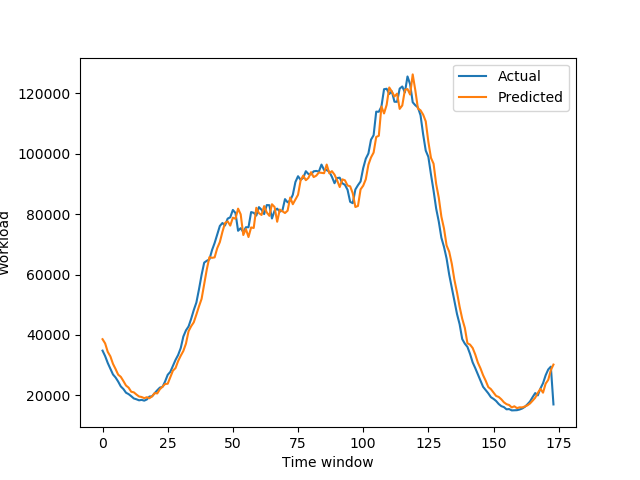
\includegraphics[width=\linewidth]{resources/baseline/arima_10.png}
      \caption{Arima prediction}
    \end{subfigure}
    \caption{Baseline predictions}
    \label{fig:baseline_pred}
  \end{figure}

  \subsubsection{ARIMA}
  ARIMA\cite{arima}, which stands for autoregressive integrated moving average, is a classic approach 
  to modelling timeseries. In order to apply this model we need to find appropiate values for its 
  parameters: p, q, d. 
  
  The value of d means the number of times the series needs to be differentiated
  in order to make it stationary. The series stationarity was checked using the augmented Dickey-Fuller 
  test\cite{Dickey-Fuller} which found the p-value to be 1.0902496274664773e-08. This is lower than 0.05, 
  the commonly used threshold, meaning we can set d to 0. 
  
  The partial autocorrelation plot was analyzed
  to set the autoregression parameter (p). From figure \ref{fig:arima_params} we can see that the significance
  region is confidently passed at 1, with a steep decline afterwards. The moving average parameter (q) is 
  approximated from the autocorrelation plot. It suggests a value of around 20 would be a good start. 
  After fitting ARIMA(1,0,20) the final 2 layers had P-value of 0.547 and 0.758 which meant that they were 
  not significant. After trying some values for q: 5,10,15,18 the best results were obtained on ARIMA(1,0,15)
  with 14263566.564, MAE: 3056.765, MAPE: 6.349.

  \begin{figure}
    \centering
    \begin{subfigure}[b]{0.4\linewidth}
      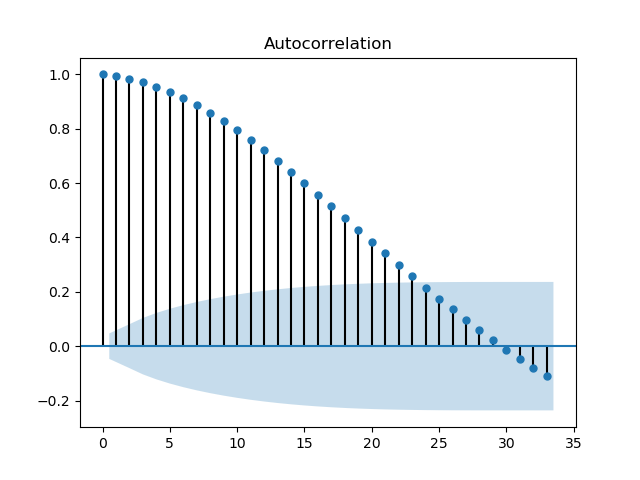
\includegraphics[width=\linewidth]{resources/baseline/arima_10_acf.png}
      \caption{Autocorrelation plot}
    \end{subfigure}
    \begin{subfigure}[b]{0.4\linewidth}
      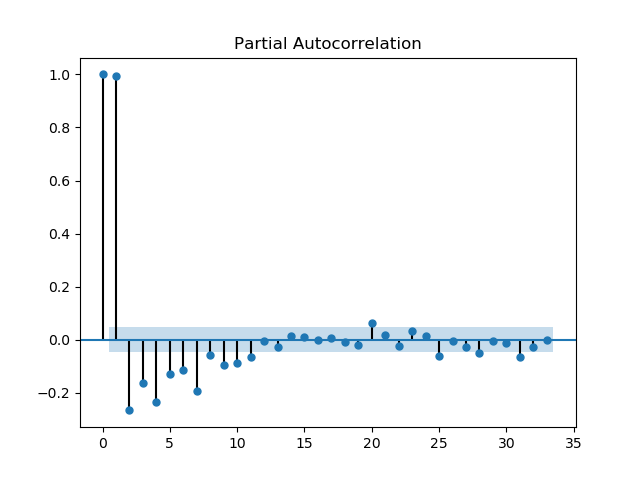
\includegraphics[width=\linewidth]{resources/baseline/arima_10_pacf.png}
      \caption{Partial autocorrelation plot}
    \end{subfigure}
    \caption{ARIMA params}
    \label{fig:arima_params}
  \end{figure}

  \subsection{Deep learning models}

  \subsubsection{MLP}
  After some manual experiments started with a MLP with 2 hidden layers (150, 100 neurons) and sliding window
  size of 24 (input size). 

  To find an optimal combination of batch size and epoch no a 2d grid search was performed \ref{fig:epoch_batch}.
  Batch size should ideally be a power of 2 for extra perfromance on GPU architectures, as some 
  experiments were ran on Google Colab. Lower batch size is more accurate but training is slower\cite{batch_size}.
  As expected the best MSE is obtained for the lowest batch size(4) however it does not drop significantly
  at 8, regardless of epochs no. The selection of epoch no is again a tradeoff between speed and accuracy. 
  We see a smaller no of epochs(50) performs poorly, while the difference between 100 and 250 is not that great,
  meaning that we can get a good approximation of a model using a batch size of 100.

  \begin{figure}
    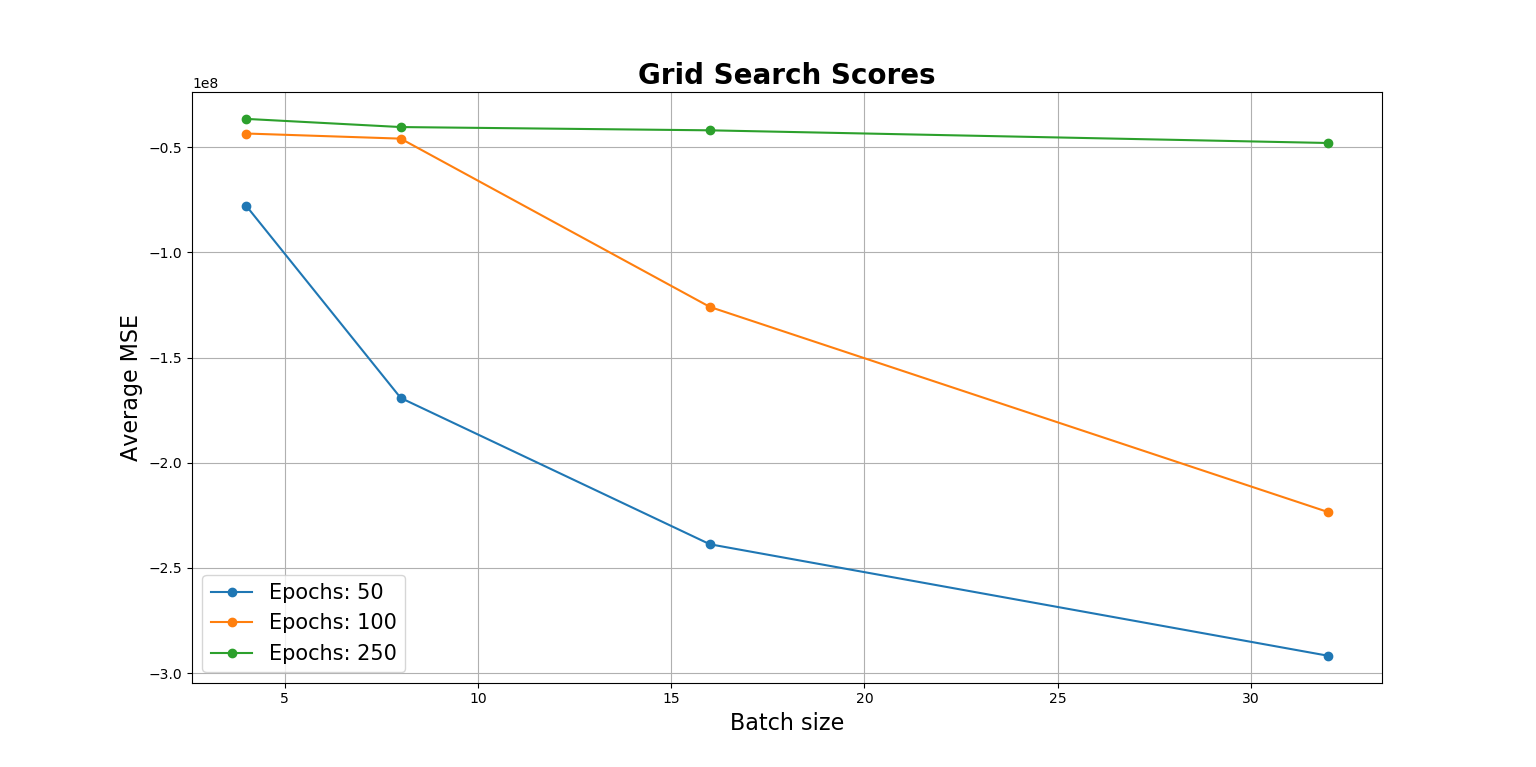
\includegraphics[width=\linewidth]{resources/mlp/epochs_batch.png}
    \caption{2d grid search for epoch no and batch size}
    \label{fig:epoch_batch}
  \end{figure}

  Some experiments were done with adding Dropout layers on different values (0.2, 0.1, 0.05) however it did 
  not improve performance. These are generally used to prevent overfitting, when the network is too big, the 
  data is scarce or training is done for too long\cite{dropout}, which was not the case for this experiment.

  Various optimizer and activation functions were tested. The Adadelta optimizer and the 
  relu activation were selected. A comprehensive grid search was performed for sliding window size and number 
  and content of hidden layers, of around 90 combinations. Some of the best performing are presented 
  in table \ref{tab:layers}.

  \begin{table}
    \caption{Selecting optimizer and activation. Scores are averaged MSE.}
    \begin{minipage}{.5\linewidth}
      \caption*{Optimizer}
      \centering
        \begin{tabular}{ll}
            RMSprop & 24734800\\
            Adadelta & 19291753\\
            Adagrad & 190604349\\
            Adam & 25828119\\
            Adamax & 29578706\\
            Nadam & 20400557
        \end{tabular}
    \end{minipage}%
    \begin{minipage}{.5\linewidth}
      \centering
        \caption*{Activation function}
        \begin{tabular}{ll}
            softmax & 4875804739\\
            softplus & 20314197\\
            softsign & 4034049993\\
            relu & 19571788\\
            tanh & 4175933232\\
            sigmoid & 3055609656\\
            linear & 20661311
        \end{tabular}
    \end{minipage}
  \end{table}

  \begin{table}
    \begin{center}
      \caption{MLP layers and size tuning}
      \label{tab:layers}
      \begin{tabular}{c|c|c}
        \textbf{Sliding window} & \textbf{Layers} & \textbf{MSE}\\
        \hline
        4 & (100, 50, 25, 20, 10) & 18889414\\
        4 & (10, 10, 10, 10, 10, 10) & 18935098\\
        4 & (100, 50, 50, 20, 10) & 18847516\\
        8 & (100, 50, 25, 20, 10) & 17044955\\
        8 & (150, 50, 50, 50, 50, 10) & 17216134\\
        8 & (50, 50, 50, 50) & 18394493\\
        16 & (10, 20, 30, 40, 50) & 18116299\\
        16 & (100, 20, 20, 20, 10) & 18466524\\
        16 & (10, 10, 10, 10, 10, 10, 10) & 18311036\\
      \end{tabular}
    \end{center}
  \end{table}

  \subsubsection{CNN}
  Firstly, a baseline model was selected through manual experimentation. This had the following structure:
  intput of size 20, a 1d convolutional layer, a maxpooling layer, a flatten layer, a dense layer of size 150 
  and the output layer. The same batch size, epoch no grid search was performed and it yielded similar results 
  to \ref{fig:epoch_batch}. This was followed by iterating the same optimizers and activation function in 
  order to select Adadelta and softplus. 

  \begin{table}
    \begin{center}
      \caption{CNN layers and size tuning}
      \label{tab:layers_cnn}
      \begin{tabular}{c|c|c}
        \textbf{Sliding window} & \textbf{Layers} & \textbf{MSE}\\
        \hline
        8 & (25, 10, 5) & 35385451\\
        64 & (100, 20, 10, 5) & 35012864\\
        128 & (100, 20, 10, 5) & 21086942\\
        128 & (300, 50) & 22287266\\
        128 & (10, 10, 10) & 23441869\\
        256 & (100,20,10,5) & 23783826\\
      \end{tabular}
    \end{center}
  \end{table}

  The main idea behind using a CNN model for this task is to pass a larger history window as input. 
  CNN layers build different filter that learn certain characteristics of the input data. They are well 
  suited for data which has a spatial relationship(like timeseries)\cite{cnn}.

  \subsubsection{CNN-LSTM Hybrid}
  This model was applied on a range of timeseries tasks by Lin et al.\cite{cnn_lstm}.
  The starting values for 
  some parameters were influenced by this research: 32 cnn filters, 1 lstm layer with 
  a couple hundred units.

  \begin{table}
    \begin{center}
      \caption{CNN-LSTM layers and size tuning}
      \label{tab:layers_cnn_lstm}
      \begin{tabular}{c|c|c}
        \textbf{Sliding window} & \textbf{LSTM layers} & \textbf{MSE}\\
        \hline
        144 & (20, 10, 5) & 51700082\\
        todo & todo & todo\\
      \end{tabular}
    \end{center}
  \end{table}


  \subsection{Experiment Results}

  Each of the most promising models were then trained again on all training data,
  for a larger number of epochs and repeated multiple times to account for the 
  random weight initialization. The best results were then compared to baselines
  and to eachother as seen in table \ref{tab:final_eval}.

  \begin{table}[h]
    \begin{center}
      \caption{Final results}
      \label{tab:final_eval}
      \begin{tabular}{c|c|c|c|c|c}
        \textbf{Dataset} & \textbf{Naive} & \textbf{ARIMA} & \textbf{MLP} & \textbf{CNN} & \textbf{CNN-LSTM} \\
        \hline
        Jp10 & 20233320 & 15289199 & 8591086 & 12766376 & 7252806 \\
        Jp15 & 87883950 & 56662039 & 31042348 & 36278866 & 57719162 \\
        De10 & 16789198 & 10318406 & 5180340 & todo & todo \\
        De15 & 77481580 & 43398336 & 17276322 & todo & todo \\
      \end{tabular}
    \end{center}
  \end{table}

  \section{For article - REMOVE ME}
  \section{Data preparation}
  The raw data used for this experiment is a wikipedia 
  trace for 12 days in september 2007\cite{wikidata}. 
  From this a subset of requests was 
  extracted as separate datasets: all requests to Japanese and German wikipedia
  respectively. 
  The subsets were selected 
  in order to compare results with Kim et al.\cite{CloudInsight} which used 
  the same data. Another reason for extracting subsets it's that the 
  amount of data after preparation is the same as what we would extract from the global
  trace, given it's the same time range,
  but processing is much faster.

  In order to turn a web request log file into a supervised dataset the following steps were,
  taken: 
  \begin{itemize}
  \item extract timestamps of all requests for a country (e.g. all lines matching ja.wikipedia)
  \item create buckets which contain the number of requests in a
  time interval
  \item iterate over the buckets using the sliding window technique\cite{sliding_window}, described below
  \end{itemize}
  
  The starting point for the sliding window is a time series 
  $(t_1, t_2, .., t_{size})$
  where $t_i$ is the number of requests in the i-th bucket.
  Training instances are then generated with input 
  $(t_{i}, t_{i+1}, ... t_{i+n-1})$
  and output $(t_{i+n+1})$, 
  where n is the size of the sliding window. 
  This process starts at i = 1 and is incremented by 1 until i = size - n + 1. 
  The predicted value is $t_{i+n+1}$ instead of $t_{i+n}$ because a scaler using this model 
  would need to have a buffer window during which to deploy the services.

  \begin{figure}
    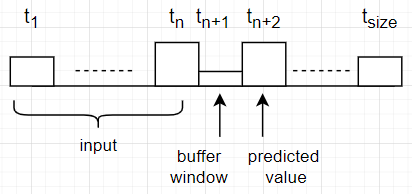
\includegraphics[width=\linewidth]{resources/data/prepare.png}
    \caption{Sliding window technique}
    \label{fig:sliding_window}
  \end{figure}

  The size of the datasets before applying the sliding window are 111316009 requests 
  for ja.wikipedia and 101917920 for de.wikipedia.

  \newpage
  \bibliography{bibliography}{}
  \bibliographystyle{plain}
\end{document}